\documentclass[10pt]{article}
\usepackage{fontspec}
\usepackage{amsmath,amssymb}
\usepackage{graphicx}
\usepackage{xcolor}
\usepackage{tcolorbox}
\tcbuselibrary{skins}
\usepackage{geometry}
\geometry{
    paperwidth=612.05pt,
    paperheight=720.05pt,
    top=20pt,
    headheight=14pt,
    headsep=12pt,
    bottom=28pt,
    footskip=12pt,
    left=36pt,
    right=36pt
}
\usepackage{fancyhdr}
\usepackage{tabularx}
\usepackage{multicol}
\usepackage{tikz}

\setmainfont{Times New Roman}
\setsansfont{Arial}

\definecolor{stewartcyan}{RGB}{0, 118, 186}
\definecolor{stewartred}{RGB}{218, 41, 28}
\definecolor{stewartgray}{RGB}{120, 120, 120}

\pagestyle{fancy}
\fancyhf{}
\renewcommand{\headrulewidth}{0pt}

\setlength{\abovedisplayskip}{3pt}
\setlength{\belowdisplayskip}{3pt}
\setlength{\abovedisplayshortskip}{1pt}
\setlength{\belowdisplayshortskip}{1pt}
\setlength{\parskip}{0pt}

\begin{document}
% Header
\noindent{\small\textbf{302}\qquad\textbf{\textsf{CHƯƠNG 4}}\quad Ứng dụng của đạo hàm}
\vspace{0.8em}

\setcolumnwidth{1.9in, 4.8in}
\setlength{\columnsep}{0.3in}

\begin{paracol}{2}
% Cột lề trái: Hình vẽ và chú thích
{\centering 
  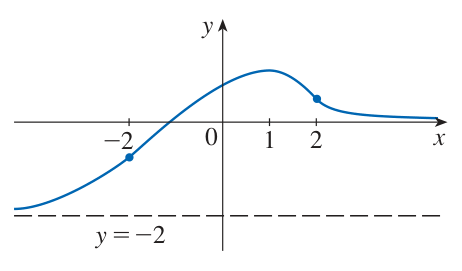
\includegraphics[width=\linewidth]{images/p0337_fig1.png}\\[4pt]
  {\small\textbf{\textsf{HÌNH 10}}}
\par}

\vspace{7.5em}

{\centering 
  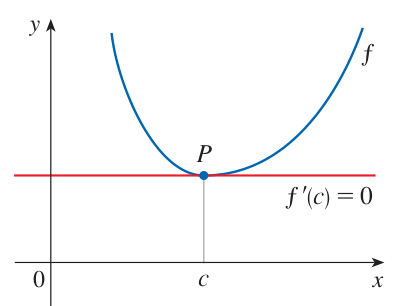
\includegraphics[width=\linewidth]{images/p0337_fig2.png}\\[4pt]
  {\small\textbf{\textsf{HÌNH 11}}}\\[2pt]
  {\footnotesize $f''(c) > 0$, $f$ lõm lên}
\par}

\switchcolumn
% Cột nội dung chính
Trước tiên, ta vẽ đường tiệm cận ngang $y = -2$ dưới dạng đường nét đứt (xem Hình 10). Sau đó vẽ đồ thị hàm số $f$ tiệm cận với đường này ở phía xa bên trái, tăng dần tới điểm cực đại tại $x = 1$, và giảm dần về phía trục $x$ ở phía xa bên phải. Chúng ta cũng cần đảm bảo rằng đồ thị có các điểm uốn tại $x = -2$ và $2$. Chú ý rằng đường cong quay bề lõm lên trên với $x < -2$ và $x > 2$, và quay bề lõm xuống dưới giữa $-2$ và $2$. \hfill{\color{stewartblue}$\blacksquare$}

\vspace{0.5em}
\noindent{\color{stewartblue}\rule{1.2ex}{1.2ex}}\hspace{0.5em}{\large\bfseries\textsf{Phép kiểm đạo hàm cấp hai}}

Một ứng dụng khác của đạo hàm cấp hai là phép kiểm sau đây nhằm xác định các giá trị cực đại và cực tiểu địa phương. Đây là hệ quả của Phép kiểm tính lõm, và đóng vai trò như một phương án thay thế cho Phép kiểm đạo hàm cấp một.

\begin{tcolorbox}[colback=white, colframe=stewartred, arc=0mm, boxrule=0.8pt, top=6pt, bottom=6pt, left=8pt, right=8pt]
  {\bfseries\color{stewartred} Phép kiểm đạo hàm cấp hai}\quad Giả sử $f''$ liên tục ở lân cận $c$.
  \begin{enumerate}[label=(\alph*), leftmargin=2em, itemsep=2pt, topsep=4pt]
    \item Nếu $f'(c) = 0$ và $f''(c) > 0$, thì $f$ đạt cực tiểu địa phương tại $c$.
    \item Nếu $f'(c) = 0$ và $f''(c) < 0$, thì $f$ đạt cực đại địa phương tại $c$.
  \end{enumerate}
\end{tcolorbox}

Chẳng hạn, mệnh đề (a) đúng vì $f''(x) > 0$ ở gần $c$ và do đó $f$ lõm lên ở gần $c$. Điều này có nghĩa là đồ thị của $f$ nằm \emph{phía trên} tiếp tuyến nằm ngang của nó tại $c$ và vì vậy $f$ đạt cực tiểu địa phương tại $c$. (Xem Hình 11.)

\vspace{0.3em}
\noindent{\bfseries\textsf{\color{stewartblue}LƯU Ý}}\quad Phép kiểm đạo hàm cấp hai không đưa ra kết luận khi $f''(c) = 0$. Nói cách khác, tại một điểm như vậy có thể có cực đại, có thể có cực tiểu, hoặc không có cực trị nào cả. Phép kiểm này cũng không áp dụng được khi $f''(c)$ không tồn tại. Trong các trường hợp đó, ta phải dùng Phép kiểm đạo hàm cấp một. Trên thực tế, ngay cả khi cả hai phép kiểm đều áp dụng được, Phép kiểm đạo hàm cấp một thường dễ dùng hơn.

\vspace{0.4em}
\noindent{\bfseries\textsf{\color{stewartblue}VÍ DỤ 6}}\quad Khảo sát đường cong $y = x^4 - 4x^3$ về tính lõm, các điểm uốn, cùng các điểm cực đại và cực tiểu địa phương.

\vspace{0.2em}
\noindent{\bfseries\textsf{\color{stewartblue}LỜI GIẢI}}\quad Nếu $f(x) = x^4 - 4x^3$, ta có
\begin{align*}
  f'(x) &= 4x^3 - 12x^2 = 4x^2(x - 3) \\[2pt]
  f''(x) &= 12x^2 - 24x = 12x(x - 2)
\end{align*}
Để tìm các số tới hạn, ta giải phương trình $f'(x) = 0$ và nhận được $x = 0$ cùng $x = 3$. (Lưu ý rằng $f'$ là một đa thức nên xác định ở mọi nơi.) Để áp dụng Phép kiểm đạo hàm cấp hai, ta tính $f''$ tại các số tới hạn này:
\[
  f''(0) = 0 \qquad\qquad f''(3) = 36 > 0
\]
Vì $f'(3) = 0$ và $f''(3) > 0$, Phép kiểm đạo hàm cấp hai khẳng định rằng $f(3) = -27$ là một cực tiểu địa phương. Do $f''(0) = 0$, Phép kiểm đạo hàm cấp hai không cung cấp thông tin về số tới hạn 0. Tuy nhiên, vì $f'(x) < 0$ khi $x < 0$ và cả khi $0 < x < 3$, Phép kiểm đạo hàm cấp một cho thấy $f$ không đạt cực đại hay cực tiểu địa phương tại 0.

\end{paracol}

\vfill
{\centering 
  \tiny\color{gray}
  Copyright 2021 Cengage Learning. All Rights Reserved. May not be copied, scanned, or duplicated, in whole or in part. WCN 02-200-203
\par}

\end{document}
